\documentclass[a4paper]{article}

\title{Documentation of the R package epiphylo}
\author{Xavier Didelot}

\usepackage{Sweave}
\begin{document}
\Sconcordance{concordance:epiphylo.tex:epiphylo.Rnw:%
1 5 1 1 0 4 1 1 5 1 1 1 2 4 0 1 2 3 1 1 2 5 0 1 2 3 1 1 2 1 0 3 1 4 0 1 %
2 3 1}


\maketitle


A pathogen has an effective within-host population size of $N_e=100$ and a generation time $g=1$ day, so that the within-host coalescent rate is $N_e g=100/365$ years. The basic reproduction number is $R=1$. To following command simulates an outbreak of this pathogen: 
\begin{Schunk}
\begin{Sinput}
> simu <- simulateOutbreak(R=1,neg=100/365)
\end{Sinput}
\end{Schunk}

This simulation contains both the transmission tree between infected hosts and the within-host phlogenetic tree of each host. This can be visualised as a colored phlogenetic tree, where each host is represented by a unique color:

\begin{center}
\begin{Schunk}
\begin{Sinput}
> plotBothTree(simu)
\end{Sinput}
\end{Schunk}
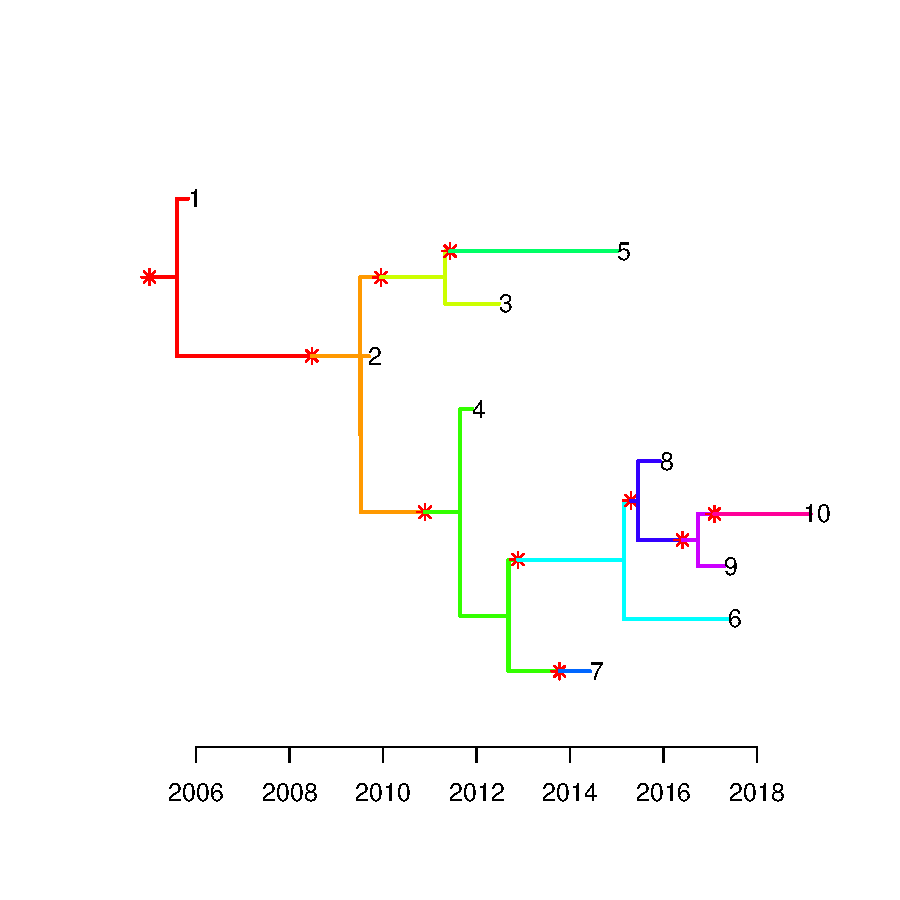
\includegraphics{epiphylo-003}
\end{center}



\end{document}
